%%%%%%%%%%%%%%%%%%%%%%%%%%%%%%%%%%%%%%%%%%%%%%%%%%%%%%%%%%%%%%%%%%%%%%%%%%%%%%%%%%%
%% This project aims to create the template for presentation.                   %%
%% author: Luigi Durso                                                          %%
%% contacts:                                                                    %%
%%    e-mail: luigi.durso@si2001.it                                             %%
%%    linktree: https://linktr.ee/maumneto                                      %%
%%%%%%%%%%%%%%%%%%%%%%%%%%%%%%%%%%%%%%%%%%%%%%%%%%%%%%%%%%%%%%%%%%%%%%%%%%%%%%%%%%%
\documentclass{../libs/presentation_format}
% Inserting the preamble file with the packages
%%%%%%%%%%%%%%%%%%%%%%%%%%%%%%%%%%%%%%%%%%%%%%%%%%%%%%%%%%%%%%%%%%%%%
%% This file contains the packages that can be used in the beamer. %%
%%%%%%%%%%%%%%%%%%%%%%%%%%%%%%%%%%%%%%%%%%%%%%%%%%%%%%%%%%%%%%%%%%%%%
% Package to fonts family
\usepackage[T1]{fontenc}
% Package to accentuation
\usepackage[utf8]{inputenc}
% Package to Italian language
\usepackage[italian]{babel}
% Package to Figures
\usepackage{graphicx}
\usepackage{caption}
\usepackage{subcaption}
% Package to the colors
\usepackage{color}
% Package to the colors
\usepackage{xcolor}
% Packages to math symbols and expressions
\usepackage{amsfonts, amssymb, amsmath}
% Package to multiple lines and columns in table
\usepackage{multirow, array} 
% Package to create pseudo-code
% For more detail of this package: http://linorg.usp.br/CTAN/macros/latex/contrib/algorithm2e/doc/algorithm2e.pdf
\usepackage{algorithm2e}
% Package to insert code
\usepackage{listings} 
\usepackage{keyval}
% Package to justify text
\usepackage[document]{ragged2e}
% Package to manage the bibliography
\usepackage[backend=biber, style=numeric, sorting=none]{biblatex}
% Package to facilities quotations
\usepackage{csquotes}
% Package to use multicols
\usepackage{multicol}
% Inserting the references file
\bibliography{../references.bib}

% Title
\title[Flutter-Dart]{\huge\textbf{Flutter e Dart - Le basi}}
% Subtitle
\subtitle{Flutter - Applicazioni adaptive e responsive}
% Author of the presentation
\author{Luigi Durso}
% Company's Name
\institute[SI2001]{
    % email for contact
    \normalsize{\email{luigi.durso@si2001.it}}
    \newline
    \centering
    
\includegraphics[scale=0.3]{../libs/emblem.png}
    \newline
    % company name
    \company
}
% date of the presentation
\date{\today}


%%%%%%%%%%%%%%%%%%%%%%%%%%%%%%%%%%%%%%%%%%%%%%%%%%%%%%%%%%%%%%%%%%%%%%%%%%%%%%%%%%
%% Start Document of the Presentation                                           %%               
%%%%%%%%%%%%%%%%%%%%%%%%%%%%%%%%%%%%%%%%%%%%%%%%%%%%%%%%%%%%%%%%%%%%%%%%%%%%%%%%%%
\begin{document}
% insert the code style
%%%%%%%%%%%%%%%%%%%%%%%%%%%%%%%%%%%%%%%%%%%%%%%%%%%%%%%%%%%%%%%%%%%%%%%%%%%%%%%%%%%
%% This file contains the style of the codes show in slides.                     %%
%% The package used is listings, but it possible to used others.                 %%
%%%%%%%%%%%%%%%%%%%%%%%%%%%%%%%%%%%%%%%%%%%%%%%%%%%%%%%%%%%%%%%%%%%%%%%%%%%%%%%%%%%

% color used in the code style
\definecolor{codegreen}{rgb}{0,0.6,0}
\definecolor{codegray}{rgb}{0.5,0.5,0.5}
\definecolor{codepurple}{rgb}{0.58,0,0.82}
\definecolor{codebackground}{rgb}{0.95,0.95,0.92}

% style of the code!
\lstdefinestyle{codestyle}{
    backgroundcolor=\color{codebackground},   
    commentstyle=\color{codegreen},
    keywordstyle=\color{magenta},
    numberstyle=\tiny\color{codegray},
    stringstyle=\color{codepurple},
    basicstyle=\ttfamily\footnotesize,
    frame=single,
    breakatwhitespace=false,         
    breaklines=true,                 
    captionpos=b,                    
    keepspaces=true,                 
    numbers=left,                    
    numbersep=5pt,                  
    showspaces=false,                
    showstringspaces=false,
    showtabs=false,                  
    tabsize=2,
    title=\lstname 
}

\lstset{style=codestyle}

\lstset{basicstyle=\ttfamily,
	showstringspaces=false,
	commentstyle=\color{red},
	keywordstyle=\color{blue},
	inputencoding=utf8,
	extendedchars=true
}


%% ---------------------------------------------------------------------------
% First frame (with tile, subtitle, ...)
\begin{frame}{}
    \maketitle
\end{frame}

%% ---------------------------------------------------------------------------
% Table of content frame
\begin{frame}{Sommario}
    \begin{multicols}{2}
        \tableofcontents
    \end{multicols}
\end{frame}

%% ---------------------------------------------------------------------------

\section{Lezione precedente}
\begin{frame}{Un po' di codice}
\begin{tabular}{lll}
	\raisebox{-.5\height}{
\includegraphics[scale=0.3]{../libs/Developer-Friendly.png}}
	\emph{Analizziamo l'elaborato precedente!}\\
\end{tabular}
\end{frame}

%% ---------------------------------------------------------------------------

\section{Responsive}
\begin{frame}{Cosa vuol dire responsive}
\begin{figure}[htpb]
		\centering
		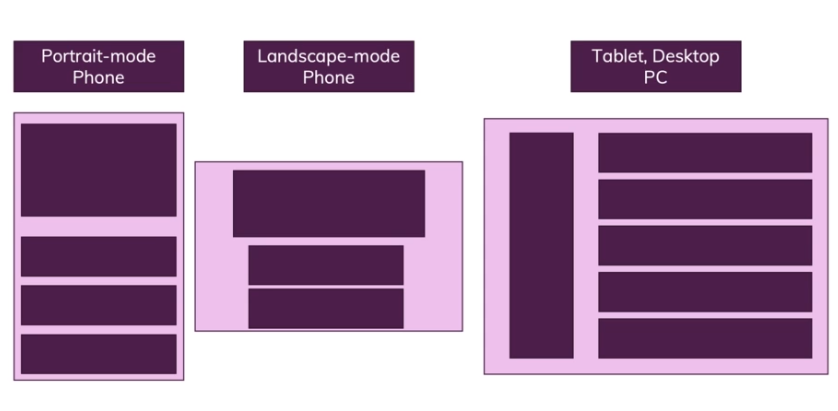
\includegraphics[width=9cm]{../libs/responsive-overview}
	\end{figure}
\end{frame}

%% ---------------------------------------------------------------------------

\begin{frame}{Flexible Widget}
	\emph{Un widget che ci è molto utile nella creazione di UI responsive è sicuramente il \emph{Flexible Widget}:}
	\begin{itemize}
		\item Controlla la modalità di riempimento degli spazi dei figli;
		\item Da combinare con widget come Column, Row, Flex
		\item Si può usare il Widget \emph{Expanded} per ottenere il risultato di un Flexible con fit tight
	\end{itemize}
\end{frame}

%% ---------------------------------------------------------------------------

\begin{frame}{Misure dinamiche}
	\emph{Inserire delle misure statiche può non essere il modo giusto per la creazione di UI Responsive:}
	\begin{itemize}
		\item Possiamo calcolare dinamicamente le misure assegnate ai nostri widget
		\item Un'ottima base per il calcolo delle misure è sicuramente lo spazio disponibile a schermo
		\item Recuperiamo dal contesto le misure del nostro display attraverso \emph{MediaQuery}
		\item Altra informazione molto utile recuperabile da MediaQuery è \emph{L'orientation} del dispositivo
	\end{itemize}
	\centering
	\emph{Attenzione!} MediaQuery richiama automaticamente la rebuild ad ogni suo cambiamento!
\end{frame}

%% ---------------------------------------------------------------------------

\begin{frame}{Layout Builder}
	\begin{minipage}[0.2\textheight]{\textwidth}
		\begin{columns}[T]
			\begin{column}{0.4\textwidth}
				\begin{figure}[htpb]
					\centering
					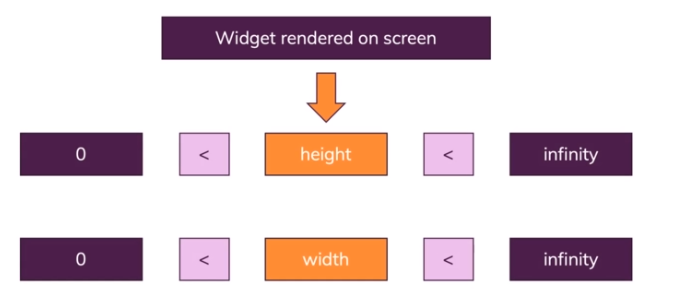
\includegraphics[scale=0.2]{../libs/constraints-layout}
				\end{figure}
			\end{column}
			\begin{column}{0.6\textwidth}
				\emph{Uno strumento per controllare lo spazio disponibile:}
				\begin{itemize}
					\item Widget che permette di sfruttare lo spazio disponibile, spazio definito dal padre esplicitamente oppure implicitamente
					\item Controllo effettuato attraverso l'uso dei constraints
					\item Nei constraints abbiamo le info su ampiezza ed altezza disponibili
					\item I constraints sono implicitamente utilizzati ogni volta che definiamo delle misure, oppure utilizziamo widget che ne fanno uso. \emph{Es. Expanded}
				\end{itemize}
			\end{column}
		\end{columns}
	\end{minipage}
\end{frame}

%% ---------------------------------------------------------------------------

\section{Adaptive}
\begin{frame}{Diverse piattaforme}
	\emph{Essendo Flutter di natura cross-platform, abbiamo strumenti per gestire diverse piattaforme:}
	\begin{itemize}
		\item Possiamo creare widget \emph{Adattivi} che vengono renderizzati in modo differente in base alla piattaforma in uso
		\item Molti widget integrano un costruttore \emph{.adaptive} che permette di gestire il multi-piattaforma
		\item Per individuare la piattaforma possiamo usare la classe \emph{Platform} di dart.io
	\end{itemize}
\end{frame}

%% ---------------------------------------------------------------------------

\begin{frame}{Cupertino widget}
	\emph{Flutter non è solo Material Design}
	\begin{itemize}
		\item Diamo una occhiata ai widget basati su uno stile "ios-centrico"
	\end{itemize}
	\centering
	\href{https://docs.flutter.dev/development/ui/widgets/cupertino}{\beamergotobutton{Documentazione}}
\end{frame}

%% ---------------------------------------------------------------------------

\section{Esercitazione}
\begin{frame}{Migliorare la precedente esercitazione}
	\begin{minipage}[0.2\textheight]{\textwidth}
		\begin{columns}[T]
			\begin{column}{0.4\textwidth}
				\begin{figure}[htpb]
					\centering
					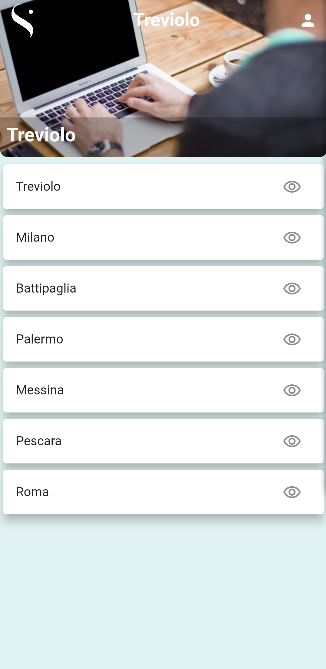
\includegraphics[width=2cm]{../libs/assignment-2-home}
				\end{figure}
			\end{column}
			\begin{column}{0.6\textwidth}
				\emph{Alcuni spunti:}
				\begin{itemize}
					\item Utilizzare i widget Flexible ed Expanded dove possibile,
					\item Sfruttare MediaQuery e Costraints per l'assegnazione delle sizes
					\item Disegnare in versione \emph{Landscape} un dettaglio sulla sede corrente ( uno spunto in foto
				\end{itemize}
			\end{column}
		\end{columns}
	\end{minipage}
\end{frame}


%% ---------------------------------------------------------------------------

% Reference frames
\begin{frame}[allowframebreaks]
    \frametitle{Riferimenti}
    \printbibliography
\end{frame}

%% ---------------------------------------------------------------------------
% Final frame
\section{Fine}
\begin{frame}{}
	\huge\emph{Grazie per l'attenzione!}
	\newline
	\vfill
	\hfill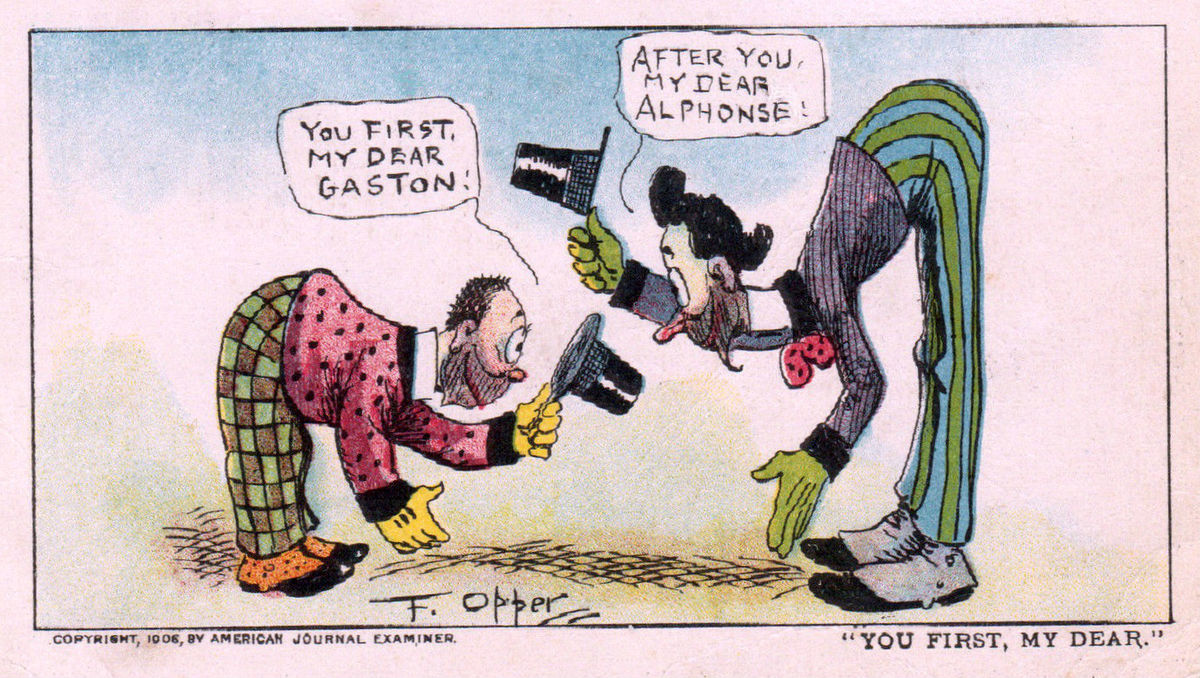
\includegraphics[width=6cm]{../libs/alphonse-gaston-regards}
\end{frame}

\end{document}